\section{Diseño de interiores}
\subsection{Definicion}
El diseño de interiores es una profesión en la cual soluciones creativas y técnicas son aplicadas dentro de una estructura para lograr la construcción de un entorno interno determinado. Éstas soluciones son funcionales, mejoran la calidad de vida de los ocupantes y son aestéticamente atractivas. Los diseños deben apegarse al código y normas requisitados, y fomentar los principios de sustentabilidad ambiental definidos por el edificio o empresa. El objetivo del diseño de interiores es lograr una armonía en los espacios que habitamos y dar confort al usuario de dichos espacios.\cite{B01} \par
El diseño de interiores sigue una metodología sistemática y coordinada que incluye investigación, análisis e integración de conocimientos dentro de un proceso creativo. Dentro ésta metodología podemos ubicar distintos servicios o etapas, dependiento de la complejidad del trabajo, en las cuales encontramos: definición de los requerimientos funcionales para los espacios de las habitaciones, planeación de espacios interiores, realización de planos de construcción, definición de especificaciones de ubicación, colores y acabados en piso, paredes, materiales, equipo, mobiliario y muebles, administración de contratos de fabricación o instalación, etc.\par
En Estados Unidos el diseño de interiores es la única rama del diseño que está sujeta a las regulaciones federales y la ley gubernamental.\cite{B02}
\subsection{El diseño de interiores a través de la historia}

\subsubsection{Mid Century Modern}
\subsubsection{Feng shui}
\subsubsection{Deconstructivismo}
\subsubsection{Diseño Orgánico}

\subsection{Fundamentos del diseño de interiores}
El diseño de interiores se ve como una actividad que tiene un punto de inicio (cuando el diseñador y el cliente tienen el primer contacto) y otro al final cuandl el proyecto se ha ejecutado.\par
Se debe tomar en cuenta que el diseño de interiores es maleable, es decir, que su realización no está sujeto estrictamente a una serie de reglas. En un caso se puede realizar un determinado proceso, y en otro se puede realizar otro proceso diferente. No existe una solución estandarizada para para todos los casos.\par
Lo más importante es definir el por qué estamos diseñando. Por ejemplo si se está diseñando un armario, se tiene qué saber cuál es el impulso para hacerlo. El diseñador se plantea algunas ideas sobre las funciones que tiene un armario, el uso de la madera, reciclada, el del plástico o el nuevo material, y con base a eso, define el objetivo de diseñar el armario.
Otro fundamento importante es la armonía que se busca. Un espacio interior no sólo debe verse bonito, y tener colores agradables a la vista. Cada elemento que compone un espacio debe relacionarse con los demás. Un sillón en una sala de espera debe relacionarse y tener alguna conexión con la mesa de centro. Esta relación puede ser la similitud del acabado de ambos, la ubicación de uno con respecto al otro, etc.
Una habitación debe seguir un esquema de colores bien definido. Dentro de estos esquemas tenemos el monocromático, complementario y análogo, y cada uno deriva del círculo cromático.\par

\textbf{Monocromático}.- Es una selección de colores que funcionen bien juntos. Esto es trabajar con un matiz, y la variación de tintes, tonos, y sombras.
\begin{figure}[h!]
	\centering
	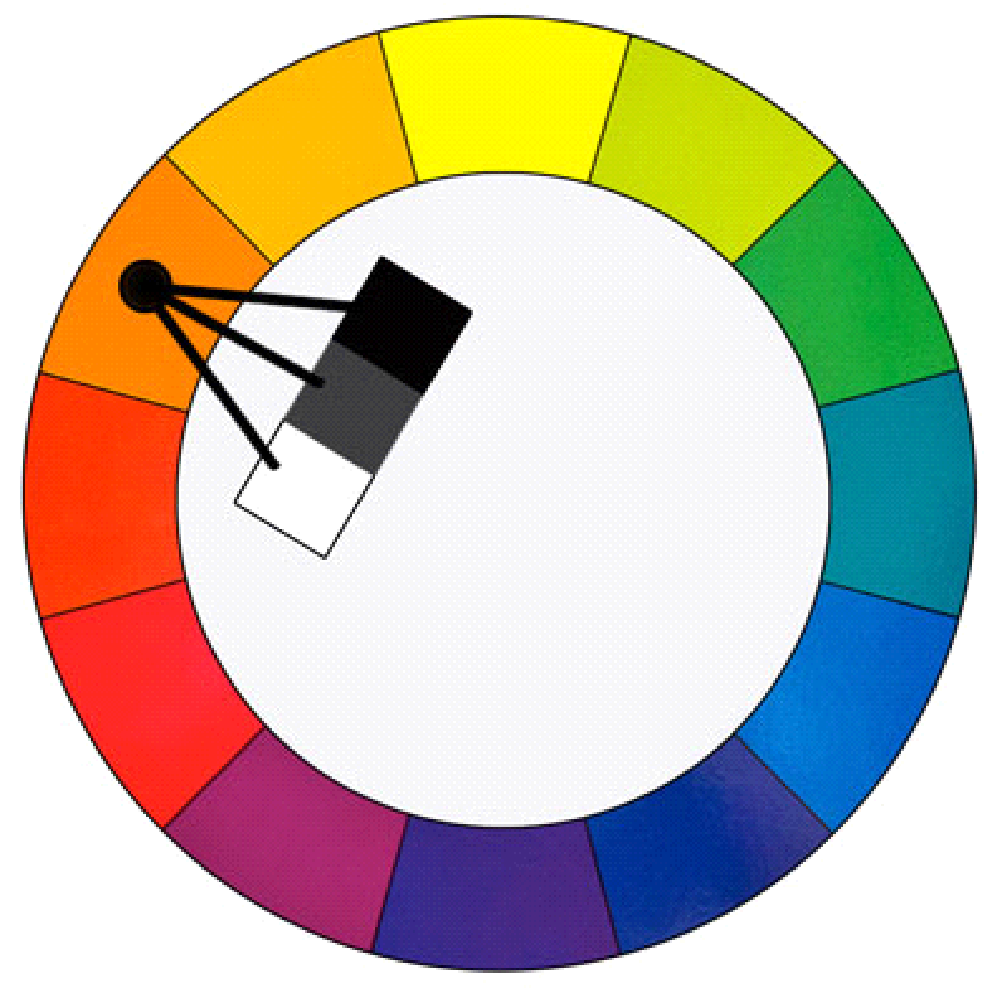
\includegraphics[width=7cm]{imagenes/marcoteorico/disenointeriores/monocromatico.png}
	\caption{Esquema monocromático.\cite{B13}}
	\label{fig:monocromatico}
\end{figure}

\textbf{Complementario}.- Los colores que se encuentran en extremos opuestos del círculo cromático se consideran complementarios. Al combinar estos dos colores, se puede expresar contraste e interés. Son difíciles de usar en grandes cantidades, pero por su contraste son muy buenos para resaltar algo, como un llamado de atención.
\begin{figure}[h!]
	\centering
	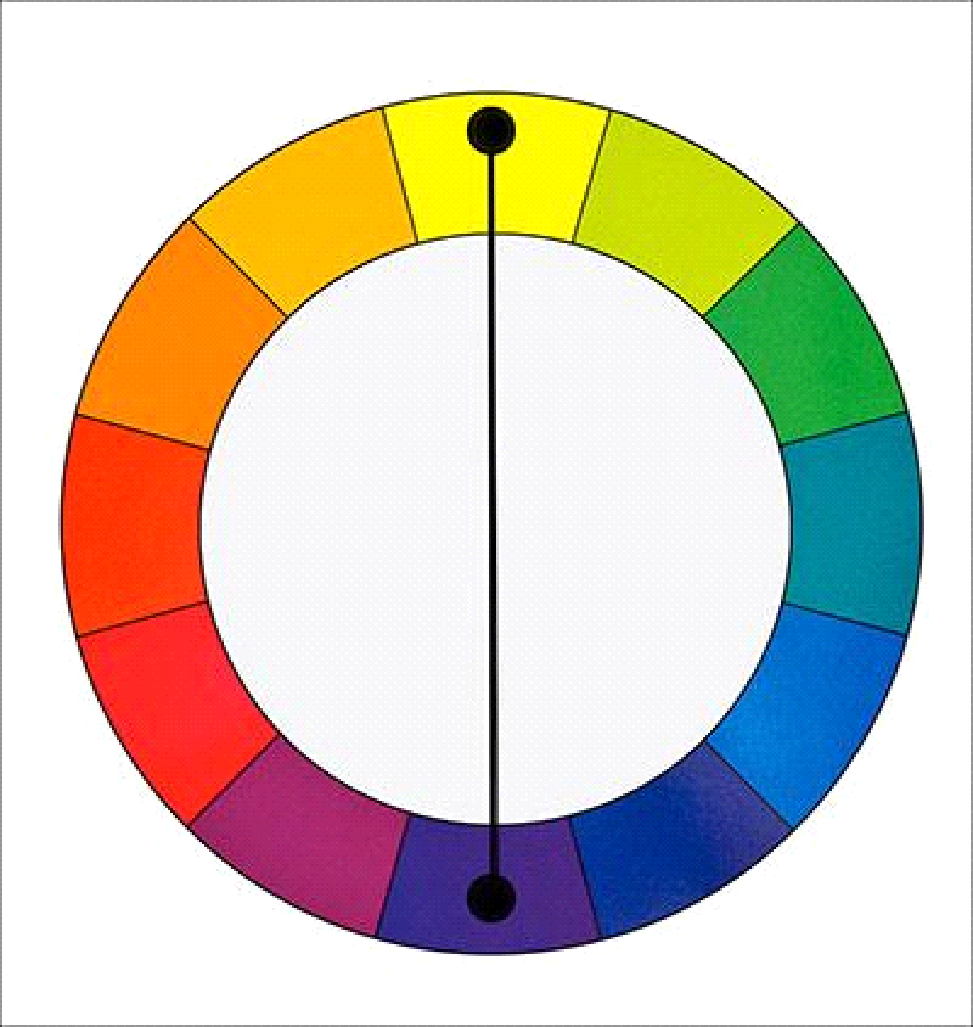
\includegraphics[width=7cm]{imagenes/marcoteorico/disenointeriores/complementario.png}
	\caption{Esquema complementario.\cite{B13}}
	\label{fig:complementario}
\end{figure}

\textbf{Análogo}.- Los colores que se encuentran al lado en el círculo cromático, son agradables juntos. Son la combinación perfecta, ya que son perfectos para cualquier uso, incluso para resaltar y contrastar un elemento específico sin demasiada interrupción. Como regla general, se debe seleccionar un color dominante, un segundo color para sustentar, y un tercer color para acentuar.\cite{B13}
\begin{figure}[h!]
	\centering
	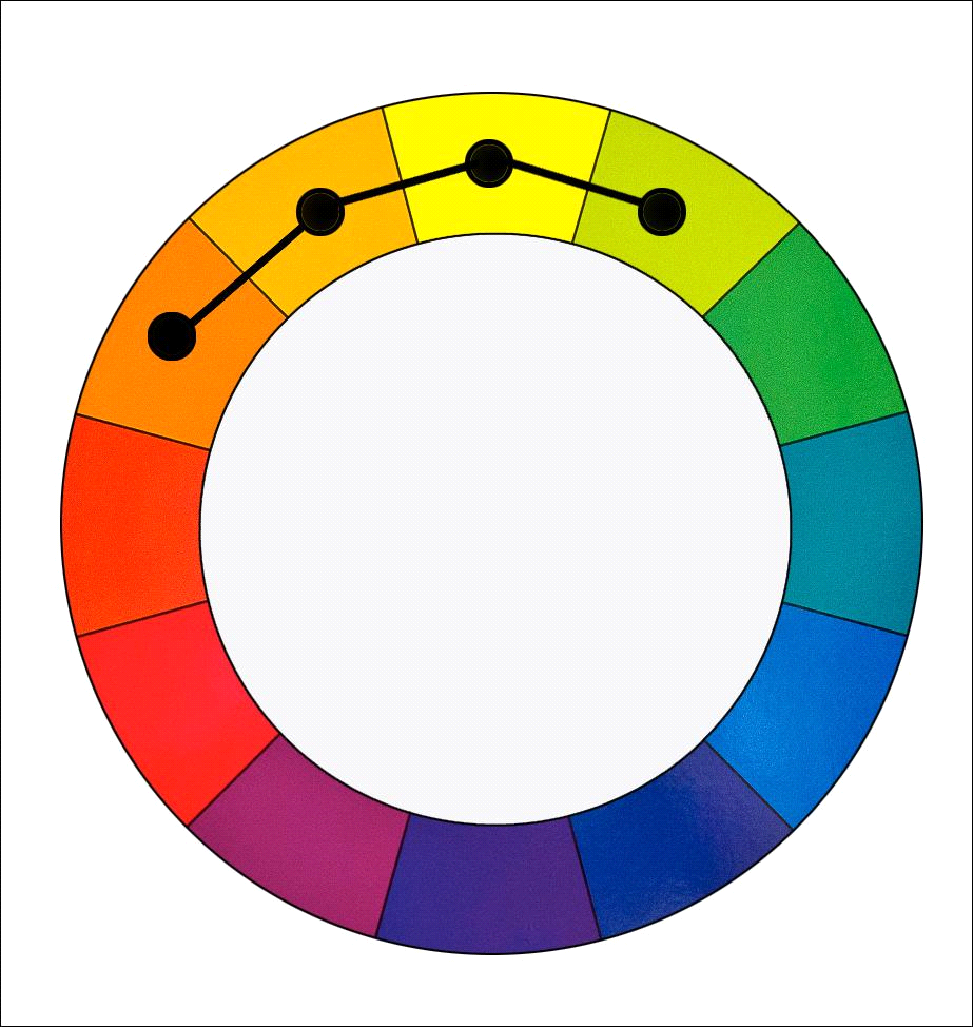
\includegraphics[width=7cm]{imagenes/marcoteorico/disenointeriores/analogo.png}
	\caption{Esquema análogo.\cite{B13}}
	\label{fig:analogo}
\end{figure}


\par 
